\documentclass[a4paper,oneside, 12pt]{article}
\usepackage[english, romanian]{babel}
\usepackage[utf8]{inputenc}
\usepackage{pdfpages}
\usepackage{listings}
\usepackage{xcolor}
\usepackage[margin=0.5in]{geometry}
\usepackage{textcomp}
\usepackage{color}
\usepackage{pdflscape}
\usepackage{hyperref}

\definecolor{codegreen}{rgb}{0,0.6,0}
\definecolor{codegray}{rgb}{0.5,0.5,0.5}
\definecolor{codepurple}{HTML}{C42043}
\definecolor{backcolour}{HTML}{F2F2F2}
\definecolor{bookColor}{cmyk}{0,0,0,0.90}  
\color{bookColor}

\lstset{upquote=true}

\lstdefinestyle{sqlstyle}{
    backgroundcolor=\color{backcolour},   
    commentstyle=\color{gray},
    keywordstyle=\color{codepurple},
    numberstyle=\numberstyle,
    stringstyle=\color{codepurple},
    basicstyle=\footnotesize\ttfamily,
    breakatwhitespace=false,
    breaklines=true,
    captionpos=b,
    keepspaces=true,
    numbers=left,
    numbersep=10pt,
    showspaces=false,
    showstringspaces=false,
    showtabs=false,
    language=SQL,
    deletekeywords={IDENTITY},
    deletekeywords={[2]INT},
    morekeywords={clustered},
    framesep=8pt,
    xleftmargin=40pt,
    framexleftmargin=40pt,
    frame=tb,
    framerule=0pt
}
\lstset{style=sqlstyle}

\newcommand\numberstyle[1]{%
    \footnotesize
    \color{codegray}%
    \ttfamily
    \ifnum#1<10 0\fi#1 |%
}

\title{Management-ul unui magazin de muzică}
\author{Nicula Ionuț-Cosmin \\ \emph{mail: }\texttt{ionut.nicula@s.unibuc.ro} \\ \emph{surse: }\texttt{github.com/niculaionut/proiect-BD}}

\begin{document}

\maketitle

\section{Descrierea modelului și a utilității acestuia}

\section{Constrângerile impuse asupra modelului}

\section{Descrierea entităților}

\section{Descrierea relațiilor}

\section{Descrierea atributelor}

\section{Diagrama entitate-relație (pagina următoare)}

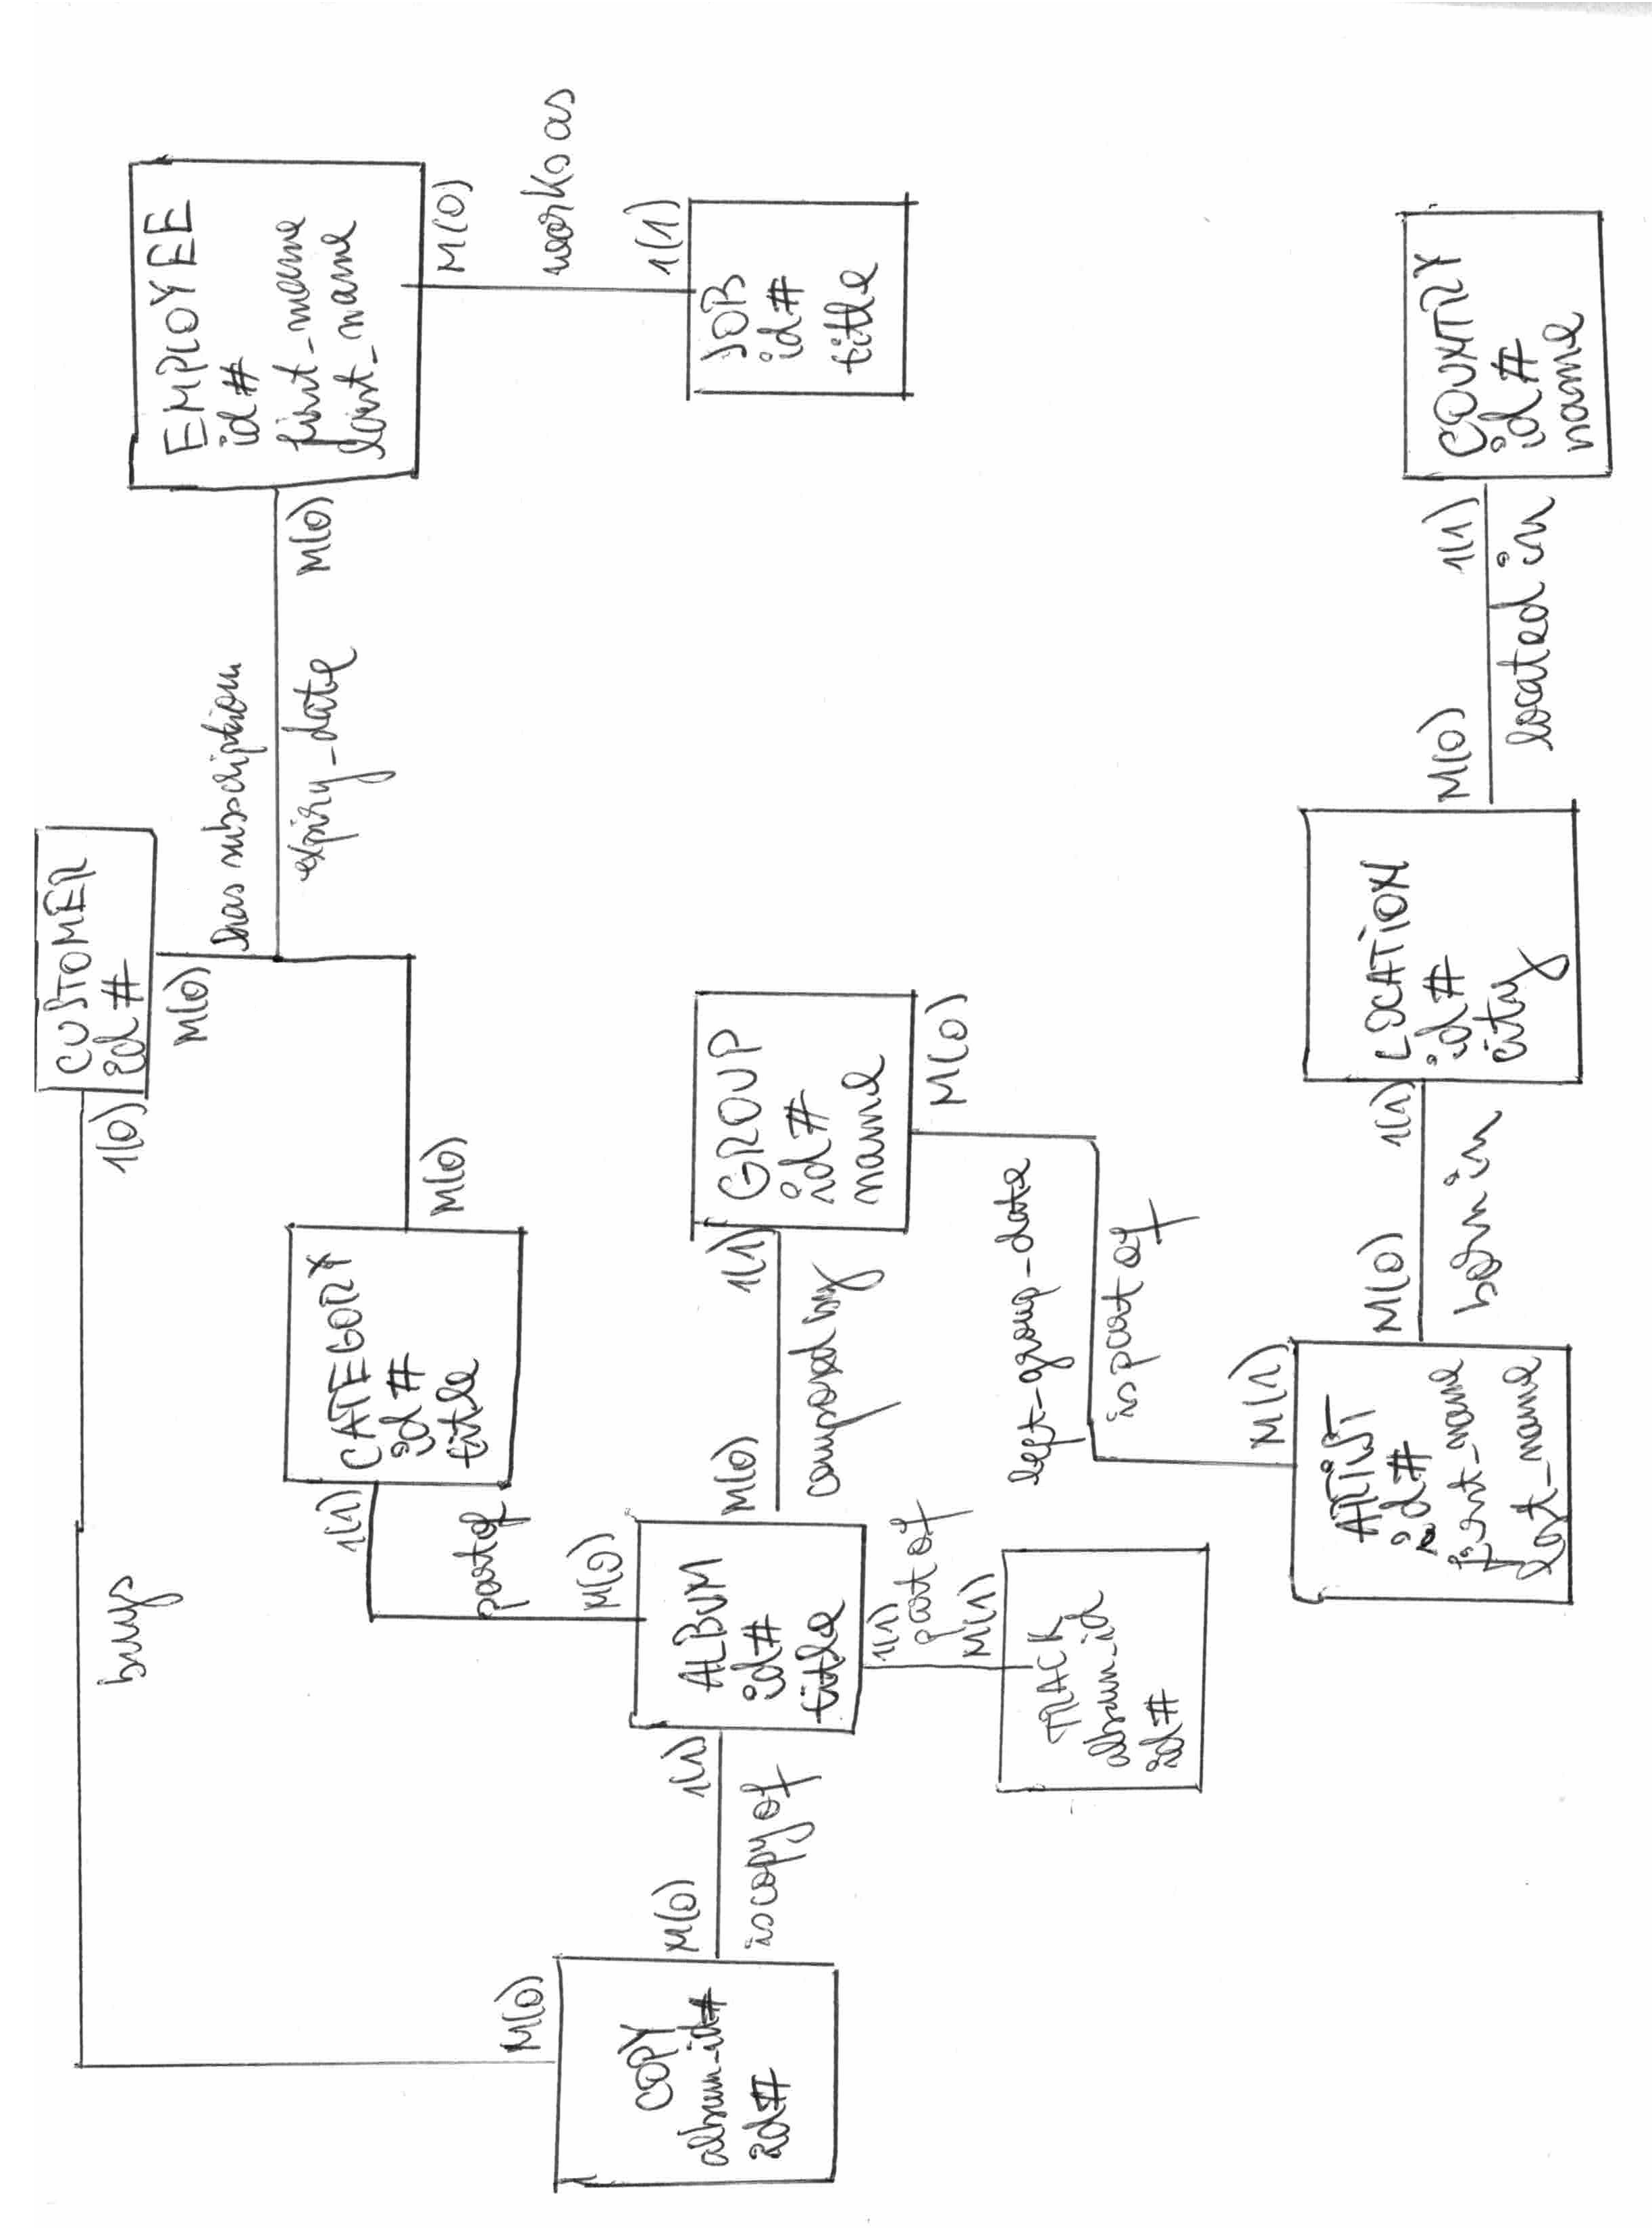
\includepdf[pages=-]{../../img/diagrama_er.png}

\section{Diagrama conceptuală (pagina următoare)}

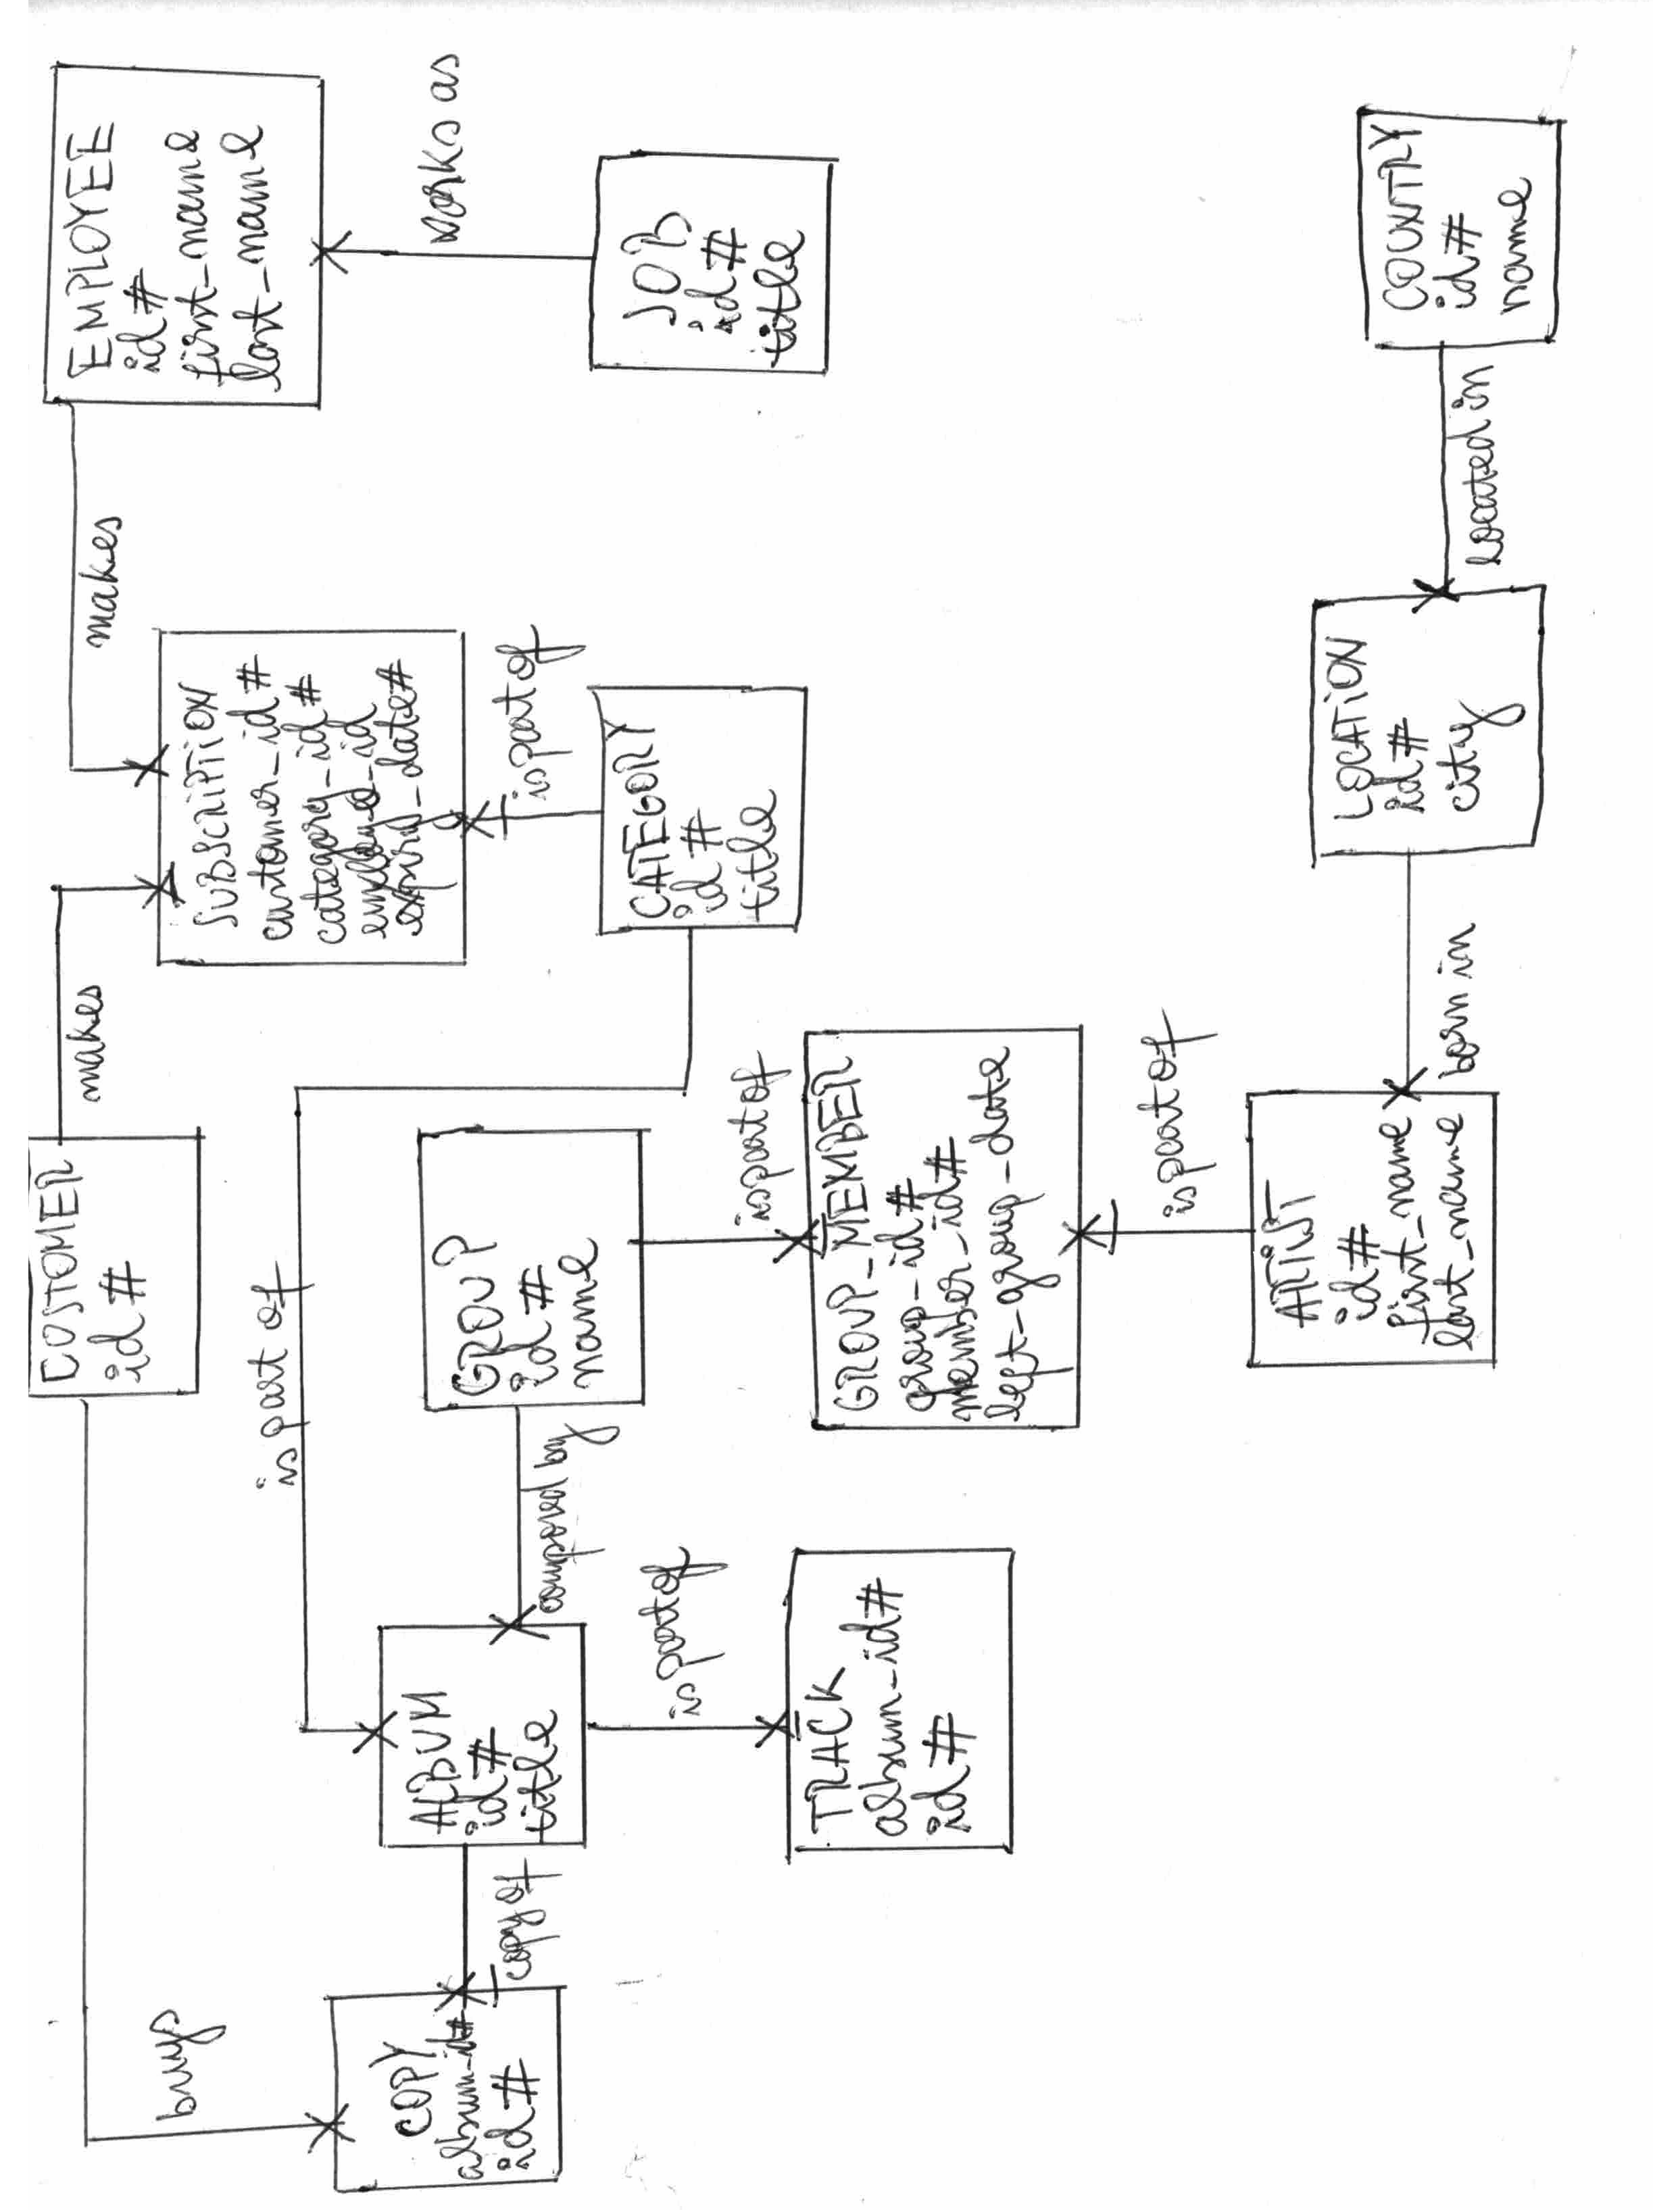
\includepdf[pages=-]{../../img/diagrama_conceptuala.png}

\section{Schemele relaționale}

\begin{center}

\lstinputlisting[language=C]{../../generate/schema_relationala.txt}

\end{center}

\section{Normalizarea până la forma normală 3}

\section{Crearea tabelelor și inserarea de date coerente}

screenshots go here

\section{Cinci cereri SQL complexe}

\begin{center}

\minipage{\linewidth}
\lstinputlisting[caption=\centering{Operație \emph{join} pe minimum 4 tabele{,} filtrare la nivel de linii{,} subcerere nesincronizată{,} ordonare{,} funcții pe șiruri de caractere}]{../../queries/1.sql}
\endminipage

\minipage{\linewidth}
\lstinputlisting[caption=\centering{Subcerere sincronizată{,} grupări{,} funcții grup{,} filtrare la nivel de grupuri{,} operații pe șiruri de caractere}]{../../queries/2.sql}
\endminipage

\minipage{\linewidth}
\lstinputlisting[caption=\textbf{NVL}{,} \textbf{DECODE}{,} \textbf{CASE}{,} funcții pe date calendaristice{,} funcții pe șiruri de caractere]{../../queries/3.sql}
\endminipage

\minipage{\linewidth}
\lstinputlisting[caption=Clauza \textbf{WITH}]{../../queries/4.sql}
\endminipage

\minipage{\linewidth}
\lstinputlisting[caption=Funcții pe date calendaristice]{../../queries/5.sql}
\endminipage

\end{center}

\section{Operații de actualizare/suprimare utilizând subcereri}

\minipage{\linewidth}
\lstinputlisting[]{../../queries/6.sql}
\endminipage

\section{Crearea unei secvențe utilizate în inserarea unor înregistrari în tabele}

\minipage{\linewidth}
\lstinputlisting[]{../../generate/create-sequence.sql}
\endminipage

\section{Cerința}
\section{Cerința}

\end{document}
